\documentclass[10pt,conference,compsocconf]{IEEEtran}

\usepackage[OT1]{fontenc} 
\usepackage{hyperref}
\usepackage{graphicx}	% For figure environment
\usepackage{subfigure}
\usepackage{titling} % Customizing the title section
\usepackage{dblfloatfix}    % To enable figures at the bottom of page
\usepackage{kantlipsum}     % for random text
\usepackage{todonotes}
\usepackage[margin=0.9in]{geometry}
\usepackage{multirow}
\usepackage[margin=0.9in]{geometry}
\usepackage[english]{babel}
\usepackage{dsfont}
\usepackage[font={small,it}]{caption}
\usepackage{array}
\usepackage{siunitx} 
\usepackage{float}
\restylefloat{table}
\usepackage{mathtools}

\begin{document}
	
\pretitle{\begin{center}\Huge\bfseries} % Article title formatting
\posttitle{\end{center}} % Article title closing formatting
\title{Bandwidth efficient object recognition for drone swarms}

\author{
	% Your name
	\textsc{Marco Zoveralli} \\
	\normalsize{Semester Project at Laboratory of Intelligent Systems} \\
	% Your supervisors
	%\textsc{Group:}
	%\normalsize{RoadSegmentationFault}\\
	% Your institution
	\normalsize \'{E}cole polytechnique f\'{e}d\'{e}rale de Lausanne
}

\maketitle
The 1-page summary goes here. This is supposed to be a 2-column per page document.
\clearpage{}

\begin{abstract}
abstract goes here
\end{abstract}

% State of the art: describe the problem and current research.
\section{Introduction}
Object detection can sometimes suffer from non-optimal viewpoints of cameras. For instance, if the angulation of a camera hides important features of an image that represents a certain object, its prediction could be wrong. The goal of this project is to improve object recognition in the context of drones swarms. In particular, we aim at making sure that, given a specific object, all the drones in the same swarm, looking at the same point, agree on the presence/absence of the object. One peculiarity of our goal consists in the fact that we want the swarm to behave as an autonomous system that is able to trigger events to more complex systems, based on whether the object is detected or not.
\subsection{Related Work}
Distributed object recognition is a problem that has been studied extensively, under different perspectives and by considering different issues.\\*
Rahimpour \textit{et al.} [REF07532441] have proposed a distributed object recognition system in the context of wireless camera networks. Their approach aims at extracting features from each camera, sending them to a base station, and delegate the whole object recognition phase to this node. The problem with this solution is that a significant amount of bandwidth is consumed -- even if their their histogram compression and feature selection framework are based on Sparse Non-negative Matrix Factorization.\\*
Medeiros \textit{et al.} [KALMANREF] have proposed an algorithm to aggregate data coming from different cameras and improve object tracking. Their protocol implies using a distributed Kalman filter in order to estimate the state. While this approach is interesting, object tracking is not our goal, since the focus of this project is object detection.\\*
Saligrama \textit{et al.} [REF01710360] have proposed an algorithm to reach a MAP (maximum a posteriori) estimate consensus in a peer to peer sensor network.\\*
Alessandro Giusti \textit{et al.} [REFHANDPREDICTION] have proposed a mechanism to perform recognition of hand gestures through a statistical classifier and distributed consensus protoco to make the nodes of the network converge to a single decision. The decision process takes into account the quality of the prediction of each node. The quality is defined as the certainty that the predicted hand gesture corresponds to the observed one. This approach is the main source of inspiration of our system, for what concerns the communication and consensus protocol. However, the setup and the goal of their solution differ from ours: they use infrared, they rely on SVM classifiers, communication, and they aim at classifying an object that they assumed to be there. Instead, we rely on wifi communication, we use neural network models, and we aim at determining whether a specified object is present or absent.
\section{System Setup}
\subsection{Hardware}
\subsubsection{Embedded boards}
The single-board computers that were used in this project were the Odroid XU4. Thanks to the high performing components of this embedded board, it is possible to run relatively complex algorithms, including neural networks. Ubuntu MATE is the chosen operating system, which allows to easily run modern software platforms, such as various Python libraries/toolkits and Go. The board has three USB interfaces and an ethernet one. Each drone will have one of these devices attached.
\subsubsection{Connectivity}
The WiFi Module 5 will be used in order to provide wifi connectivity among the Odroids boards. The choice of this component is supported by the fact that connectivity tests have shown a positive outcome for the adhoc mode too, which is the wifi mode that we use in order to make the nodes of the network communicate.
\subsubsection{Image Acquisition}
Image capture is performed by the OpenMV Cam M7 camera. It easily allows the capture of images of various sizes and their transfer to the Odroid. The connection with the board is done via USB.
\subsection{System Setup}
The initial, very simple, setup is made of three devices that join an adhoc wireless. network. Figure X shows a sketch of this configuration: the nodes communicate directly with each other and their camera points to the same direction, where the object is supposed to be. Each node runs a pre-trained neural network algorithm \footnote{\href{https://github.com/tensorflow/models/blob/master/research/object\_detection/g3doc/detection_model_zoo.md}{SSD Mobilenet}, trained on MSCOCO dataset}, thanks to the support of the tensorflow library. This model performs multiple object detection, and, in addition to the score, it also provides the bounding boxes of each prediction. Depending on the design of the consensus protocol and of the chosen setup -- which might be different from the described one --, the local prediction may be provided to one or more nodes in the network. This, along with the data aggregation phase, is described in the following section.
%The result of the local prediction of all the nodes is provided to all the other nodes in the network. Then, there is a data aggregation process, during which the nodes agree on the presence or absence of the chosen object.
%During the development phase, the hosts are reached through ethernet connections. The 
\section{Object Detection Setup}
As already mentioned, we use neural networks in order to perform object detection. Although these models perform better than several classifiers, we cannot use too complex algorithms because execution time can become an issue if we consider that each drone must do continuous predictions in order to keep its opinion up-to-date and that our single-board computers do not have the computational power of state-of-the-art clusters. Therefore, the idea is to compensate the lack of state-of-the-art networks (but still performing!) through the presence of several devices trying to detect the same object.
\subsection{Image Acquisition}
Two parameters that must be tuned during the image acquisition phase are the capture rate and the frame size.
\subsubsection{Capture rate} it defines how often images are captured and sent to the odroid board. In order to have an accurate prediction, it would be nice to have this interval as small as possible (i.e., very high rate). However, we need to make sure that our Odroids do not receive more data than they can handle: the capture rate should not be higher than the prediction rate (i.e., it does not make sense to send too many images per second if the predictions take more time), otherwise we risk of having predictions that relate to old frames, which are limited in terms of utility.
\subsubsection{Frame size} it defines how big the taken images are. Ideally, we would like to capture images whose size is similar to the ones that were used to train the dataset, in order to have better performance. However, a larger frame size implies higher computational time as well, which can have a bad impact in terms of the "capture rate vs prediction time issue".
In our setup we tested 64x64 and 128x128 images.
\subsection{Model Selection}
Among the available pre-trained models, the \href{https://github.com/tensorflow/models/blob/master/research/object\_detection/g3doc/detection_model_zoo.md}{zoo models trained with the COCO dataset} caught our attention, since they offer several alternatives in terms of performance and execution speed. We tested few of them.
It might seem that it does not make sense too perform object detection and that we could use some classifier. This is hardly true, since in any real context the captured images are quite more complex than the ones handled by classifiers: they handle simple images with one object, while in a real, complex, scenarios, we would need to detect the presence of an object that we specify among a set of items.
% someone could also argue that SSD mobilenets are at the end not that good. Surely there are better options in terms of accuracy, but they take much more time to give a result. Other alternatives usually consist in classifiers that perform far worse, since they aim at classifying an image (and as we just mentioned, it means dealing with far simples images)
\subsubsection{SSD Mobilenet}
\label{model:ssd}
Performance and computation time vary depending on the image size and on the detected object.
% 2017 model
% 64x64 images: average computation time = 100ms on pc, around 400ms on ODROID
% 128x128 images: average computation time = 120ms on pc, 400ms on ODROID
With 64x64 and 128x128 images, the average computation time on the Odroid boards is around 400ms. There is no high difference in terms of computation time, but performance is improved by 128x128 images. We can notice that with too small images there are several false negatives: although the object is clearly visible, the model is not able to detect the object or it finds it with very low confidence scores (lower than 20\%), as soon as the distance from the object slightly increases. The problem with these image sizes is that even small distances cause the detection algorithm to perform poorly, as the objects cannot be recognized and located.
One thing that we noticed about this model is that some objects are recognized better than others: for instance, people are very well detected, while objects like books are poorly detected. This should be kept in mind in case of any real use of our ideas: the model should be trained by according to what the future application is.
\subsubsection{Faster RCNN}
These models represent the state of the art in terms of accuracy. However, one big issue relates to the long prediction time, which is around 200ms on state-of-the-art hardware \ref{reference0}, and therefore it becomes unfeasable to use them on our hardware, which has much lower computational power.
\subsection{Measures of Interest}
Whenever a prediction is performed, the algorithm provides an output that contains a set of predictions. Each prediction contains the following information:
\begin{itemize}
\item the class of the object that was located.
\item the confidence score of the prediction
\item the area in which the object is located (i.e., the bounding box)
\end{itemize}
Differently from classification algorithms, here the output is not represented by a vector of probabilities whose sum is 1. In fact, object detection algorithms make several predictions on different regions, which relate to different objects and are therefore independend from each other: each chosen area has a classifier that runs in order to do a prediction that relates to the specified region.
%In order to have some insight about the validity of one host's prediction, we would like to have a probability associated to the presence of the object that the system is seeking. We can get this information if we do some reasoning on the bounding boxes that surround the objects. 
Although we do not care about object tracking, one first thought that we had, under some assumptions, was that the bounding boxes might have given some useful information in order to give proper weights to different predictions. The idea was that, if we assume that an object has symmetric features, having a larger bounding box means being closer to an object. While this makes sense, the size of the bounding box is not really related to the confidence score that the model provides. This implies that noisy predictions may cause several false negatives. This is why we are considering the confidence score as the only value for the quality of predictions. As the next section \ref{sec:design} shows, we will rely on a mechanism that considers an object as present if a subset (whose size is chosen) considers it as present.
%One assumption that we are making during this project is that the cameras in the network point to the same direction. This implies, for objects with symmetric visual features, that a larger bounding box means that the camera is closer. This gives information in terms of how influent a prediction should be. Figure YYY shows that the highest confidence is reached with a largest bounding box (i.e., smaller distance between camera and object). Alternatively, if an object is not symmetric, the bounding box may still give useful information if the angle of view is the same as the other cameras. This is shown in figure XXX: it is possible to see that the when the examined object has larger bounding box, the confidence score is higher as well. However, this would result in a setup of limited interest. Another problem is that using the bounding box as an estimate of the quality of the prediction can be risky, because the predictions are often noisy and therefore a larger bounding box is not really related to the confidence score value. Therefore, this approach is highly arguable and therefore we focused on the confidence scores given by each hosts, and we aimed at getting advantage from the numerosity of the nodes in the network -- since we are dealing with swarms of devices.
\subsection{Preliminary Object Detection Tests}
These are the object labels that we are going to consider during our experiments: person, bottle, monitor, laptop, bycicle, umbrella, skateboard, suitcase.
Preliminary experiments showed that the chosen model is able to accurately predict the presence of some kinds of objects, such as computer screens. Figure X shows that an optimal point of view allows to get a very high confidence score on this class of objects.
\section{Design}
\label{sec:design}
Designing the protocol was one of the main steps of this project. Besides being able to improve object detection, our goal is also to ensure that few bandwidth is used and that a set of devices is able to take a decision as if it was a single, independent, system. The main challenges involved are: how a single object detection prediction is obtained and how it is communicated to other hosts, what kinds of messages are transmitted, how data is aggregated and combined together, how the faults of the network nodes are handled, and how the information is transferred for external purposes.
Our protocol is divided in three different phases, that involve significantly different activities:
\begin{itemize}
\item capturing the image with the camera, and transfer it to the Odroid
\item perform object detection on the Odroid, and propagate the result to the other hosts of the network
\item aggregate information together in order to determine a final prediction
\end{itemize}
\subsection{Consensus Protocol}
Whenever a consensus problem is faced, there are few standard approaches that define how the nodes cooperate in order to achieve a result. One way consists in having a leader that takes the local predictions from all the nodes in the network, aggregates the results, takes a final decision, and propagates the final decisions to all the nodes in the network. An advantage of this approach is that the communication scheme is quite simple as well: all the nodes provide their prediction to a single node, who is the only one that needs to send replies. This also implies that the bandwidth usage is kept low, since only the leader needs to see other nodes' messages. However, this solution requires that the leader is elected dynamically in case of failures (leader election). Furthermore, there should be some criteria to determine the eligibility of nodes to become leaders (e.g. the node that is able to communicate with more hosts). A second approach would be to have every node to receive all the values and computing the (same) solution. While this ensures robustness (especially against faults), it also means that several unnecessary work is performed: the result is the same as the previous approach, with the difference there may be several more messages transmitted between hosts. Finally, a third approach consists in having each node to compute part of the final solution and then all the computations have to be aggregated. This approach is potentially very flexible and smart, because it allows to specify very complex data fusion mechanisms. However, these mechanisms are usually very complex and guarantee better results only with some specific assumptions. For instance, many approaches make sense if the network is separated in clusters and if each node knows who is in its cluster. Since we are assuming that in our adhoc network every node can communicate directly with all the others, we decided to proceed with the first approach.
\subsection{Protocol Overview}
\label{subsec:protooverview}
Our approach is a variant of the standard family of consensus protocols Paxos. However, our usage is different from the typical ones, which often aim to reach \textbf{state machine replication}. In fact, we want to get advantage of the hosts' predictions just to determine whether the target object is present or not. As a consequence, many of the constraints of classical consensus protocols are relaxed and do not need to be met. The idea is to define a majority as a fraction of the total number of hosts of the network (N). The majority (M) should express a meaningful lower bound in terms of number positive predictions that are needed in order to trigger a positive final prediction. We defined M=N/3 + 1.
\begin{center}
	\captionsetup{type=figure}
	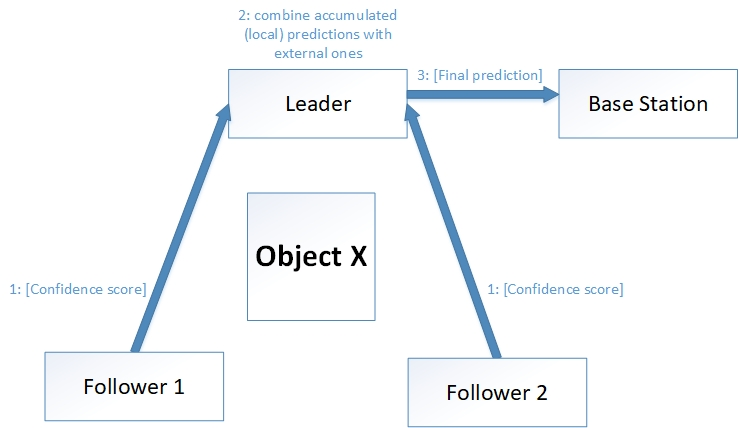
\includegraphics[width=0.47\textwidth]{img/protocol_sketch_inter_host.jpg}
	\caption {Inter-host communication}
	\label{fig:inter_host}
\end{center}
The decision process takes place in rounds: during a round there is a leader that must take a decision that is based on its local prediction and the other hosts' predictions. The leader probes all the other hosts in order to receive their predictions: the transmission of the probe message is repeated periodically (T\textsubscript{probe}) in order to compensate packet loss. Each host (including the leader) has a timeout (T\textsubscript{timeout}) after which it declares the object as absent (for that round) and it advances to the next round. T\textsubscript{timeout} = K * T\textsubscript{probe}. The leader advances to the next round after a decision for the current round is taken. This implies three cases:
\begin{itemize}
\item Timeout: the object is declared as absent for that round. This occurs if not enough positive predictions are receive or if not all predictions are received
\item Predictions from all hosts are received, but there is no positive majority: the object is declared as absent for that round.
\item A majority of positive predictions are received: the object is declared as present for that round.
\end{itemize}
\subsection{Prediction Obtainment and Inter-process communication}Once the image is captured by the camera, it is immediately transferred to the Odroid. The reason behind this choice is that the Odroid allows the usage of Linux and the Tensorflow library. This has a set of benefits, including a broad flexibility in terms choice of object detection models and language for inter-host communication.\\*
The Odroid takes care of performing object detection, through a model \ref{model:ssd} that runs over a Python process. This prediction is then forwarded to a Go process, that takes care of handling any kind of communication with the other hosts. The reason behind this choice is that Go is much more robust and flexible than Python, and its concurrency and networking features make it an excellent choice for building any kind of distributed system. This is summarized in figure \ref{fig:intra_host}:
\begin{center}
	\captionsetup{type=figure}
	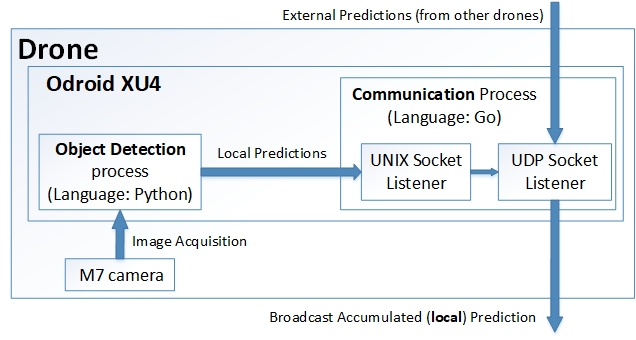
\includegraphics[width=0.47\textwidth]{img/protocol_sketch_intra_host.jpg}
	\caption {Intra-host communication}
	\label{fig:intra_host}
\end{center}
\subsection{Exchanged Messages}
There are different kinds of messages that the hosts of our system handle and propagate. They ensure that a final prediction can be obtained and sent to a base station for external usage.
\subsubsection{Probe} it is used to ask for the status of another host. A host propagating a Probe message expects a Status message as reply.
\subsubsection{Status} it is used to propagate the status of the host that forwards the message. The status include the round in which the sending host is, and the current local prediction that relates to the presence/absence of the target object.
\subsubsection{Final Prediction} it contains the final prediction, after considering the other hosts' predictions as well.
\subsubsection{Acknowledgement} a message for confirming the reception of a Final Prediction message.
\subsubsection{Start Round} a message for forcing another host to start a new round. It contains the ID of the round that has to be started.
\subsection{Communication Strategy}We decided to use connectionless communication between hosts. This allows us to have a lighter communication process, because there is no need to establish and mantain communications between hosts. In order to handle faults and packet losses, each node has some timeout (described above) and resynchronization mechanism (described below).
\subsection{Propagation frequency}since each camera sends frames quite frequently (every 100ms) to the Odroid board -- which runs the object detection algorithm on each of these received frames --, having each network host propagating its decisions as soon as they are performed could cause an explosion of messages in the network. This may occur because messages are sent broadcast. Therefore, each node propagates its decision after being probed. This implies the following advantages: drones' decisions are more reliable, bandwidth usage is reduced, and the resulting protocol will indeed be simpler to handle, test and develop.
\subsection{Hosts synchronization}All the nodes that vote in the consensus must be sure that they are voting in the same consensus round as the others. In an ideal environment, with no crashes, faults, and delays, the leader should trigger the beginning of a new round for all the other hosts (with a Start Round message), after it takes a decision for the current round. However, the aforementioned events occur in a real environment. This is why the advancement to a new round can be triggered by other messages as well:
\begin{itemize}
\item Probe message: the receiver updates its status if the received message has higher Round ID that its one.
\item Status message: the receiver updates its status if the received message has higher Round ID that its one. If the received message has lower Round ID, then a probe message with the current Round ID is sent back (here the leader is trying to force the follower to update its round).
\item Start Round message: as described above, it forces an host to start a new round.
\end{itemize}
\subsubsection{Leader Election}
If we assume that all the nodes have good reachability with each other, it is not important who the leader is. Instead, it is important that the whole swarm does not rely always on the same node to be the leader, in order to avoid a single point of failure. For this reason, the leader is simply determined by the Round ID: each leader has a Node ID, and at round i, the leader is the node with Node ID = i \% N, where N is the number of hosts in our network.
\section{Experiments}
In this section we describe the results of our approach, by showing experiments performed on few well-known objects. We consider two different setups: one that involves a noisy environment and one that was performed in a clean environment without surrounding objects.
Our experiments aim to validate different aspects of our solution:
\begin{itemize}
\item communication for the consensus protocol convergence
\item data fusion mechanism
\end{itemize}
We separated the two procedures, because with the hardware that we had it was hard to validate the protocol on a real setup.
\subsection{Data Fusion Validation}
In order to validate the data fusion mechanism we compared our multi-agent system with the single-host system. The measure that we are using relates to the Precision and the Recall. Since Precision = $\frac{TP}{TP+FP}$ and Recall = $\frac{TP}{TP+FN}$, we need two different scenarios (with the same setup, in order to have consistent conditions) to evaluate them.
We assumed to be in an ideal environment. This allowed us to consider an arbitrary number of devices in order to compare the two approaches (single-host system and multi-host system). Let N be the number of hosts that we consider in our system. If N=1, we are in the special case of the single-host system. Let K be the number of different views that we consider for our experiments. For each point of view, we captured some pictures with camera while it was pointing to the object (if present, otherwise it still points to the same direction). The predictions of these pictures are aggregated in the same way as the consensus protocol does for the local prediction process.
\subsubsection{Single-host system}There are K samples (one per viewpoint), and the precision and recall are computed on the basis of the outcomes of the predictions on these samples, in the two distinct scenarios.
\subsubsection{Multi-host system}
Here, the number of samples (from which precision and recall are derived)depends on N.
We started with a noisy setup, sketched in figure XXX. 
\subsection{Communication and Consensus Test}
\subsection{Methodology}
Our approach 
\subsection{Equidistant cameras from different angulations}
As figure XXX shows, the cameras are pointing in the same direction. Depending on the nature of the object, the detection accuracy is improved in comparison of a single viewpoint prediction. 
\subsection{Not equidistant cameras from different angulations}
\section{Dataset}
\label{sec:data-analysis}
The dataset was provided by Fraunhofer-FIRST, Intelligent Data Analysis Group (Klaus-Robert M\"uller), and Freie Universit\"at Berlin, Department of Neurology, Neurophysics Group. It was first given in the "BCI competition II" (May 2003) with a sample of 416 epochs, divided in 316 train records (labeled) and 100 test records (unlabeled).
The experiment performed to create the dataset consisted in examining a normal subject sitting on a chair in a relaxed position, while he was typing on a computer keyboard in a self-chosen order. Three sessions of six minutes were taken, all conducted in the same day with a small break in-between and with an average typing speed of 1 key/second. The EEG records were made by using 28 electrodes to monitor the brain electrical activity. They measured a time slot of 500ms, ending 130ms before the key-press, with a sample frequency of 1000Hz but also provided in a downsampled version of 100Hz. In our project we used the records sampled at 100Hz, where each record is represented as a 28 (electrode's measurements) x 50 (time frames) matrix. 
An example of a record with the respective label is shown in figure~\ref{fig:Sample}.

\begin{center}
	\captionsetup{type=figure}
	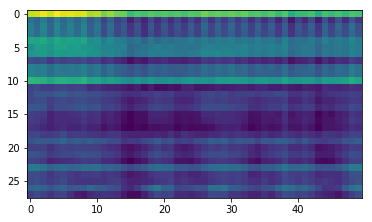
\includegraphics[width=0.5\textwidth]{img/sample.png}
	\caption {Sample from the dataset with label 1 (right movement)}
	\label{fig:Sample}
\end{center}


\section{Baseline Models}
\label{sec:baseline}
All the baseline models were tested with cross-validation and tuned with a grid search over some parameters. The input samples have been simply flattened to comply with the shape accepted by these baselines. Here we list some of the tried models, imported from the \textit{sklearn} library:
\begin{itemize}
\item \textit{Logistic Regression}. Tuned parameter: regularization. 
\item \textit{Random Forest Classifier}. Tuned parameter: max depth of the trees.
\item \textit{K-Nearest Neighbors}. Tuned parameter: K. Moreover, before training this model, we normalized the input and applied a PCA to reduce the dimensions (we kept the 95\% of the signal energy).
\end{itemize}

Table \ref{tab:baselineres} shows that none of the baselines is really able to provide a proper solution to this problem. In the next section we show the improvements that were obtained through the adoption of our own models and the methodology behind their construction. However, surprisingly, The Logistic regression model achieves good accuracy, despite the fact that it is much simpler than other models we tried.

\begin{table}[H]
\caption{Test accuracies obtained on tuned baselines.}
\label{tab:baselineres}
\centering
\begin{tabular}{ | c | c | }
\hline
Baseline & Test Accuracy \\
\hline
LogisticRegression & $70\%$ \\
\hline
Random Forest Classifier & $58\%$ \\
\hline
K-NN & $54\%$ \\
\hline
\end{tabular}
\end{table}

\section{Deep Neural Networks}
\label{sec:deep}
%We designed different models, starting from a simple Convolutional Neural Network and then tuning the parameters to reach more complex solutions.\\
%The increasing complexity of these models allowed us to get better perfomances on the test set, at the price of more time and resources needed.\\
Our methodology was based, at first, on building networks inspired to the concepts introduced during the lectures and then, we focused on tuning these models with the goal of improving the results.

%\subsection{Cross-validation}
One fundamental aspect of our approach is to perform a \textit{grid search} over a set of parameters of the network and using a \textit{cross-validation} for each combination. The cross-validation technique consists, as first step, in splitting the available train dataset in k equal parts. Then, k-1 of these sets are used to train the model and 1 is used as a validation dataset. This process is repeated k times: at each iteration, a different part is considered as validation dataset and the remaining k-1 parts are taken as training dataset. This procedure must be repeated for a set of possible values that this parameter can assume. Finally, the parameter value that lead to the best average validation score is considered as best one.

Two further issues must be taken into account. First, there are a lot of parameters that influence the score. We took into account some of the most relevant: the number of layers, the regularization terms, the type of activation functions (i.e. ReLU, Tanh, ELU) and optimizers (i.e. Adam, Adamax, Adadelta), and the number of hidden units in the last fully connected layer. However, other relevant parameters are not considered during this optimization phase. For instance, we are not iterating through the number of filters, the filter dimensions and the learning rate. Second, getting the optimal combination of parameters implies enumerating all the possible combinations of all the parameters. This results in \textit{exponential complexity} and, after some tries, we observed that this is unfeasible for our available computational resources. Therefore, we adopted an approximation of the grid search method, which consisted in a greedy approach where we selected the optimal parameters singularly and sequentially. Although this does not provide an optimal solution, it allows to keep the algorithm complexity at an acceptable level (linear). With this approach, we have to carefully choose the parameter's order. First, we search over the parameters that mostly influence the model structure, in particular the number of layers, the number of hidden units and the activation function. Then, the grid search moves to the optimizer's parameters (optimization function and weight decay) and the dropout parameter. After all the parameters are defined, we decided to perform again a search over the number of layers, as it is expected to have high influence on the performance of the model and its best value may change after the other parameters are set.
The table \ref{tab:netarch} summarizes the grid search results for all the networks.

\subsection{CNN: 2D Convolutional Layers}
The first model that we tried is a 2D Convolutional Neural Network. After a grid search on the parameters, we obtained the structure in figure \ref{fig:Conv2D}: it consists in 5 convolutional layers, ReLU as activation function and Adadelta as optimizer.

\begin{center}
	\captionsetup{type=figure}
	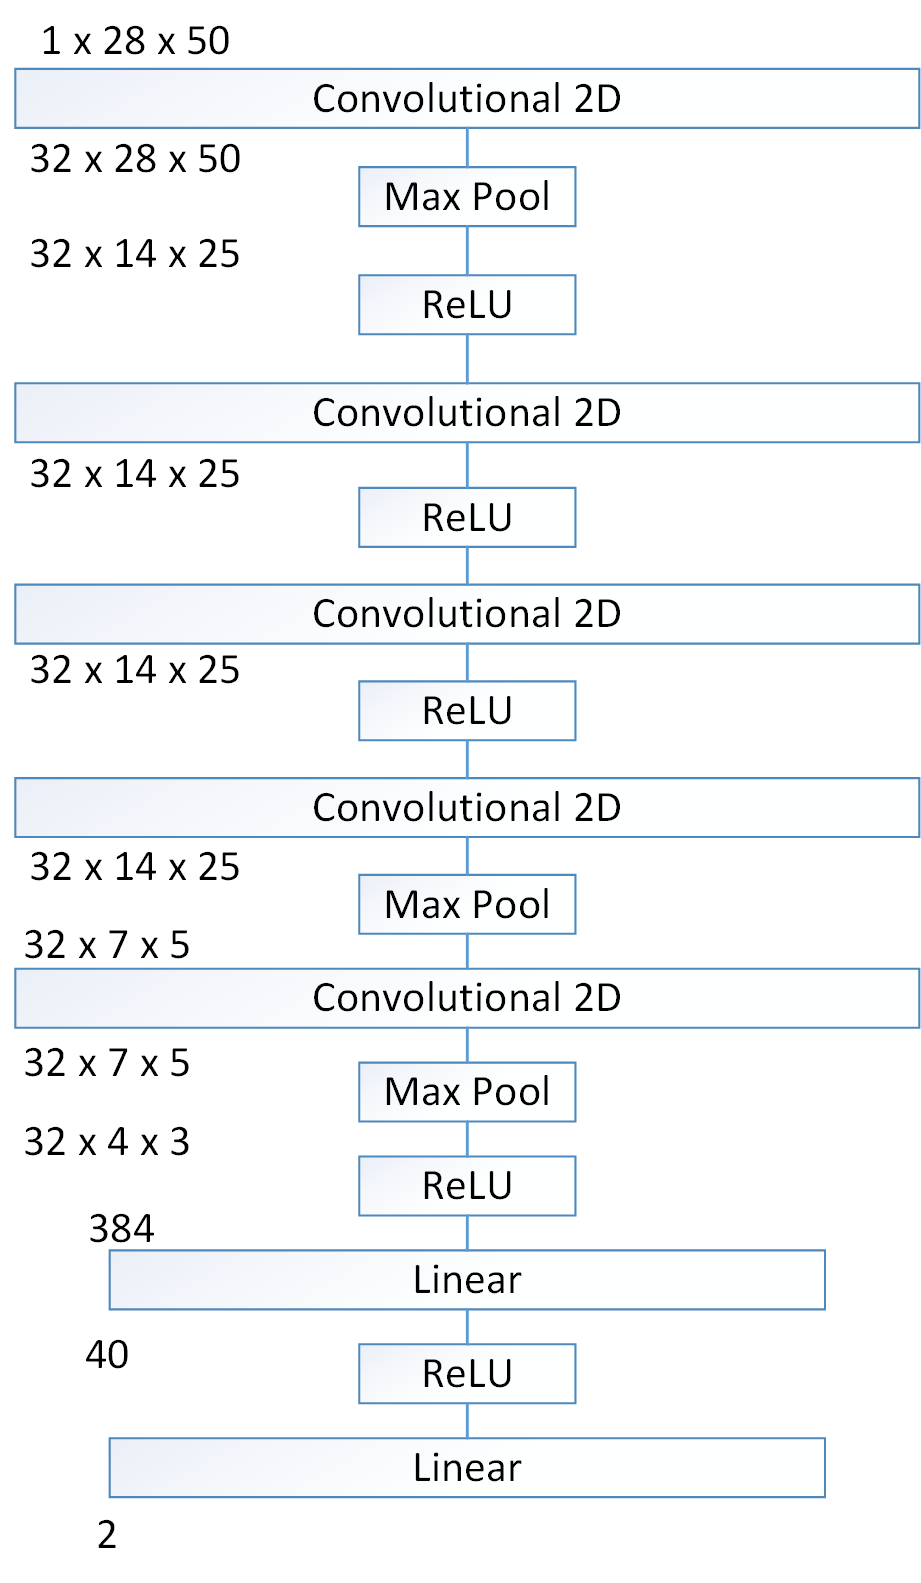
\includegraphics[width=0.35\textwidth]{img/Conv2D.png}
	\caption {2D Convolutional Neural Network}
	\label{fig:Conv2D}
\end{center}

\begin{table*}
	\caption{Network Architectures}
	\label{tab:netarch}
	\begin{tabular}{ | p{3cm} | p{2cm} | p{2cm} | p{2cm} | p{2cm} | p{2cm} | p{2cm} | }
		\hline
		Network & \#Additional Layers & \#Hidden Units & Optimizer & Activation Function & Regularization term & Dropout\\
		\hline
		A: 2D CNN
		& 3 & 40 & Adadelta & ReLU & 0.0 & 0.0 \\
		\hline
		B: 1D CNN
		& 4 & 40 & Adamax & ELU & 0.0025 & 0.1 \\
		\hline
		B: 1D CNN + Batch Norm
		& 5 & 160 & Adamax & ELU & 0.0025 & 0.3 \\
		\hline
		B: 1D CNN + Batch Norm + Dilation
		& 1 & 40 & Adamax & ELU & 0.135 & 0.1 \\
		\hline
		C:	Residual 1D CNN
		& 6 & 120 & Adamax & Tanh & 0.007 & 0.2 \\
		\hline
	\end{tabular}
\end{table*}

This network uses 2D convolutional layers, because at first it seemed natural to treat the provided dataset as a set of images. Therefore, the network was trying to find patterns between close pixels, by applying 2D filters over the input. This approach makes sense if there is a spatial relationship among the features. In our case, as mentioned in \ref{sec:data-analysis}, the input sample consists of 28 signals (EEG channels) captured over different time frames. Since the positions of the channels are not known, we cannot assume any spatial relationship between them. Therefore, applying a 2D filter over this dataset might try to find patterns between channels that are not spatially correlated. Consequently, we decided to process them all together by applying a 1D filter instead of a 2D. 


\subsection{CNN: 1D Convolutional Layers}
For the 1D CNN, we started with a simple structure and then we increased the complexity by adding more modules. In the first CNN, we only included dropout layers. Then, we used Batch Normalization, which provides significant improvements in terms of test accuracy and stability of the training. It focuses on performing normalization at each layer, and one of the main benefits is the mitigation of the change of the input distribution that may occur across the network layers. Finally, we added a dilation in the convolutional layers, hoping that increasing the receptive view of the filters could bring an improvement. Among these three variants, the best results were obtained by the 1D CNN with Batch Normalization (see Section \ref{sec:results} for the details). The structure is shown in figure \ref{fig:Conv1D}.

\begin{center}
	\captionsetup{type=figure}
	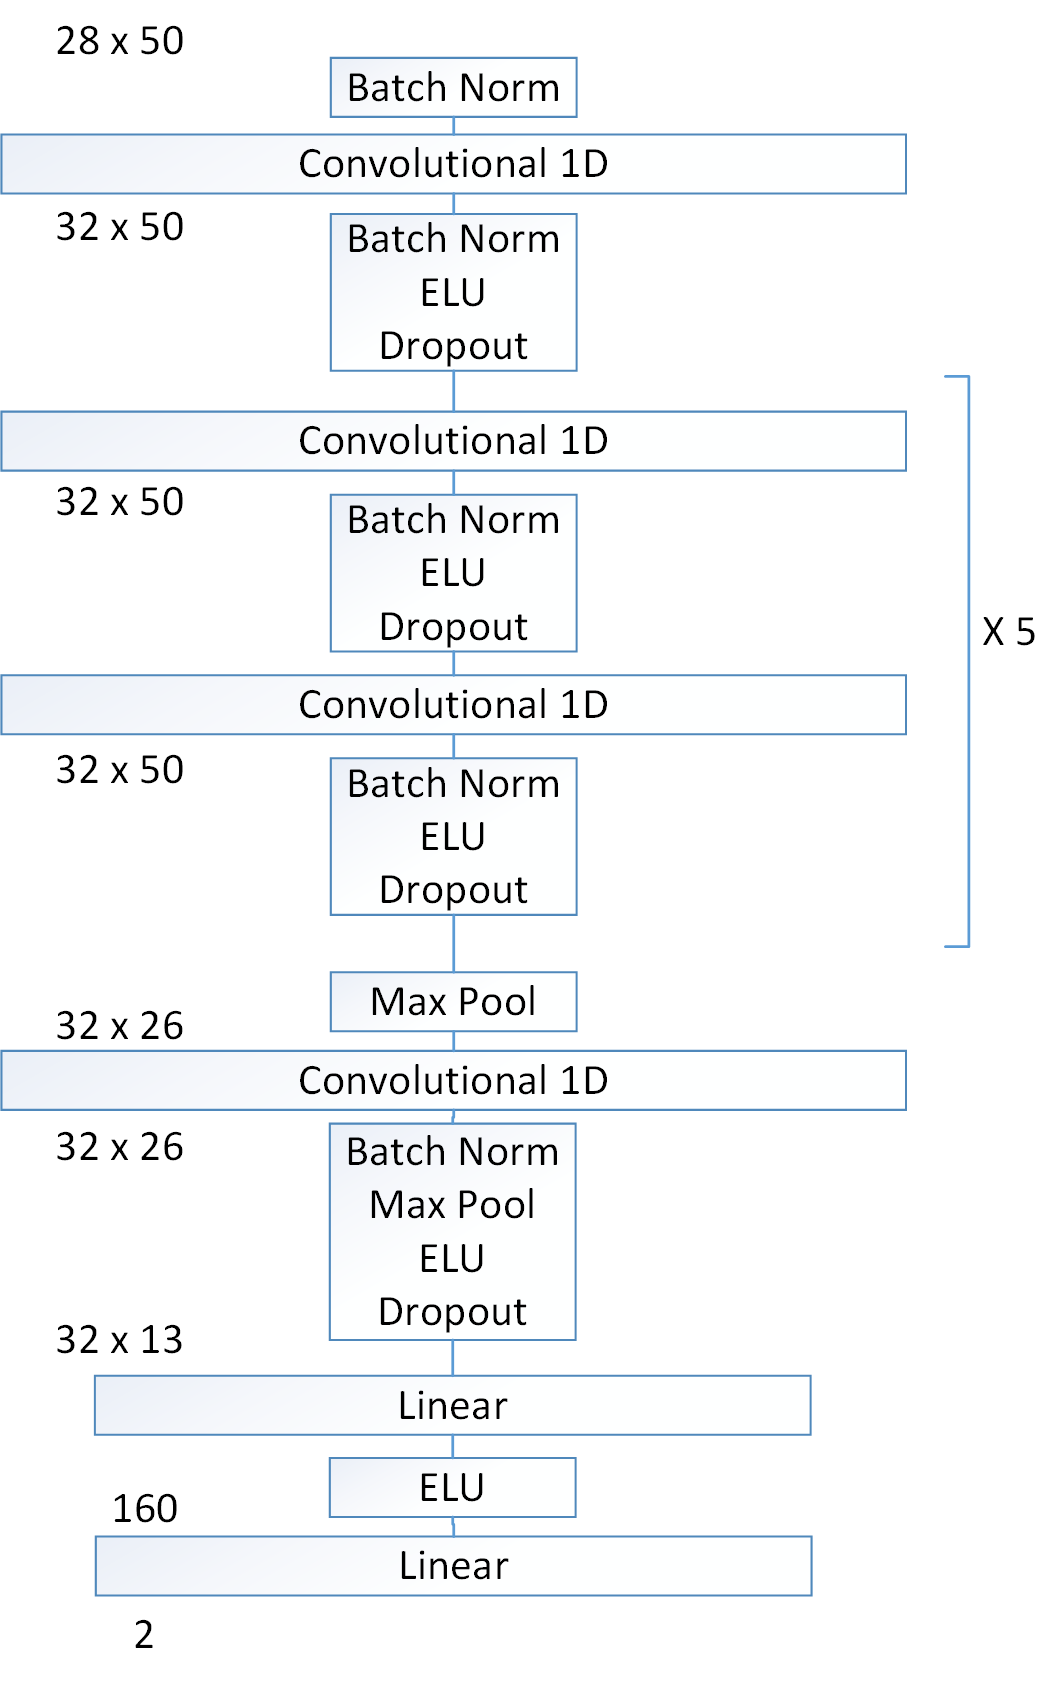
\includegraphics[width=0.37\textwidth]{img/Conv1DBatchNorm.png}
	\caption {1D Convolutional Neural Network with Batch Normalization}
	\label{fig:Conv1D}
\end{center}

One remark that concerns all the networks that involve batch normalization: although some sources\footnote{Batch Normalization: Accelerating Deep Network Training by Reducing Internal Covariate Shift - Sergey Ioffe, Christian Szegedy} claim that batch normalization makes the dropout advatanges negligible, we decided to try to tune both parameters during the grid search in any case.


\subsection{Residual 1D CNN}
This model consists in a series of aggregated residual blocks. Each residual block is made of a predefined number of convolutional layers, but the peculiarity of the block is that the input is also propagated directly to the output. Then, a group of residual blocks (two by default) are put together to construct an aggregated block. The grid search for the model iterated on the number of aggregated blocks connected sequentially. Figure \ref{fig:Residual} shows the final structure.

%A Residual CNN contains convolutional layers, linear layers, and a set of residual layers. Residual layers consist in having a block of convolutional layers (replicated a certain amount of times) whose output (at the end of the block) is influenced by the input of the block too. Our model accepts an arbitrary number of such blocks (each block has three convolutional layers), but by default there are two of them.

\begin{center}
	\captionsetup{type=figure}
	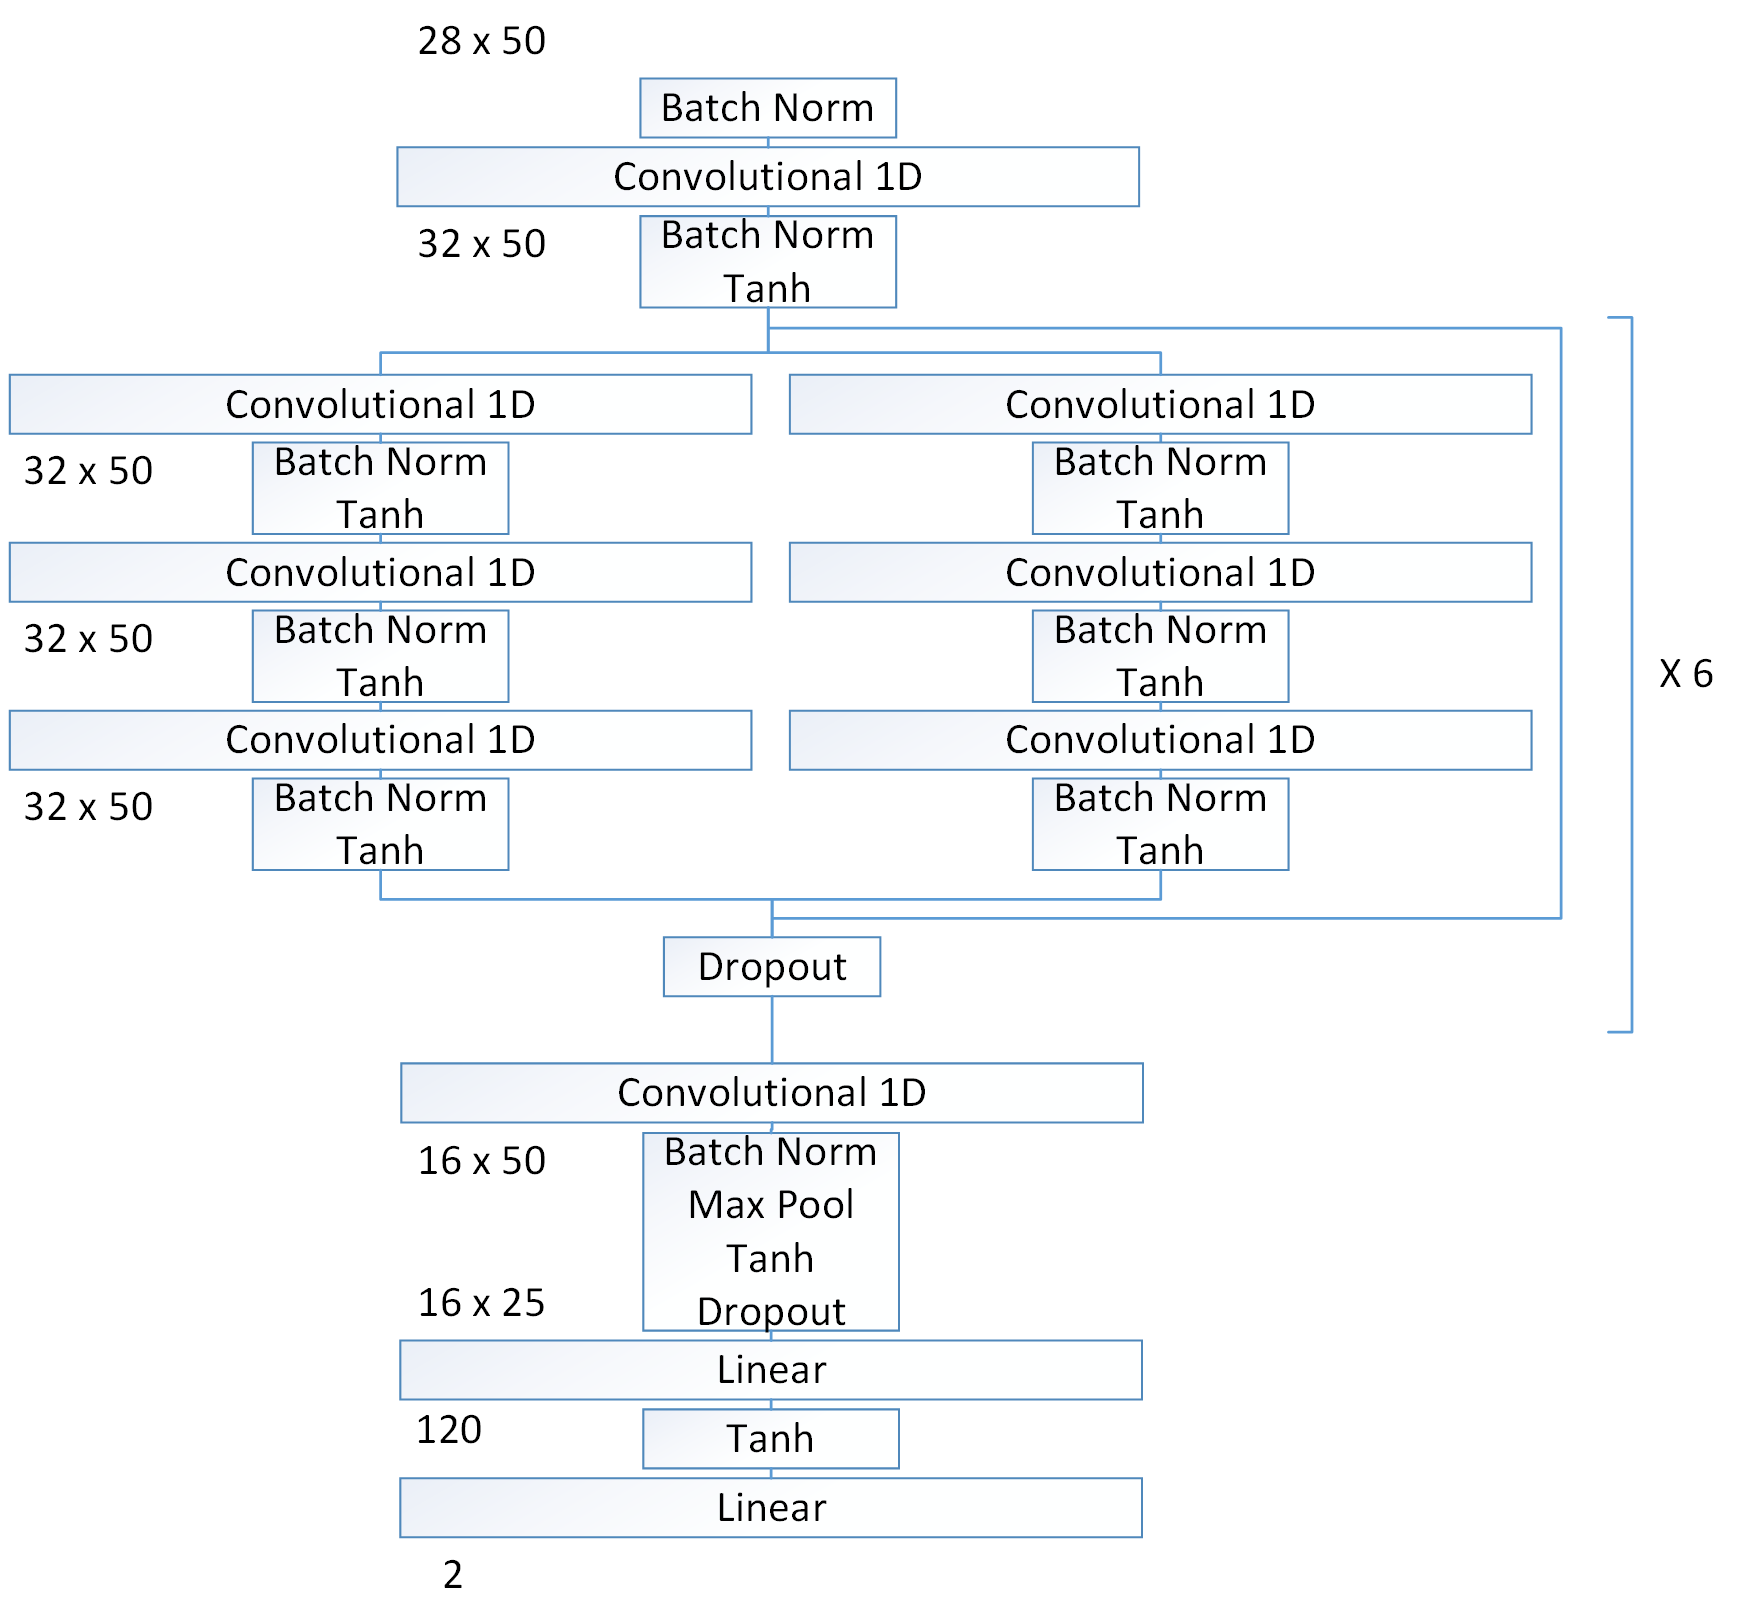
\includegraphics[width=0.5\textwidth]{img/Residual1D.png}
	\caption {1D Residual Neural Network}
	\label{fig:Residual}
\end{center}

Even if residual CNN are mainly used in the field of computer vision, we decided to try this type of network with our dataset. As we will show in section \ref{sec:results}, although the complexity of the model is much higher than the previous 1D and 2D CNN, the results did not improve in equal measure.

\section{Results}
\label{sec:results}
We now present the results of the networks that we described in the previous section. After each model has been tuned tuned with a grid search over the parameters, we tested them with a cross-validation on the train set and with a final evaluation over the test set. Figure \ref{fig:CrossVal} shows the results of the cross-validation.

We can notice that the loss function decreases faster and with more stability when using the Adamax optimizer.

\section{Conclusion}
\label{sec:conclusion}
The results that we obtained are partially satisfying. On one hand, the test accuracy is not excellent. The reasons can be found in the limited size of the train and test set and in the fact that no preprocessing was performed. Understanding the nature of the input signal was beyond the goal of this project, but an accurate analysis on the EEG dataset could have led to better results.

Still, the methodology that we followed allowed us to improve the models at each step and compare them in order to select the expected best one. The limitation of the computational power forced us to apply an approximation of the grid search technique. It can be argued that an extensive search on the parameters could have given an higher accuracy for all the models.


\begin{thebibliography}{1}
\bibitem{IEEEhowto:kopka}
\label{reference0}
Shaoqing Ren, Kaiming He, Ross Girshick, and Jian Sun \emph{Faster R-CNN: Towards Real-Time Object
Detection with Region Proposal Networks}, June 2015.
\bibitem{IEEEhowto:kopka}
\vspace*{-0.8\baselineskip}
\label{reference1}
Wei Liu, Dragomir Anguelov, Dumitru Erhan, Christian Szegedy, Scott Reed, Cheng-Yang Fu, and Alexander C. Berg \emph{SSD: Single Shot MultiBox Detector}, December 2016.
\bibitem{IEEEhowto:kopka}
\vspace*{-0.8\baselineskip}
\label{reference2}
Andrew G. Howard, Menglong Zhu, Bo Chen, Dmitry Kalenichenko, Weijun Wang, Tobias Weyand, Marco Andreetto, and Hartwig Adam \emph{MobileNets: Efficient Convolutional Neural Networks for Mobile Vision Applications}, April 2017.
\end{thebibliography}



\end{document}
